%   File: robot_moment.tex
% Author: Adam Leeper (with modification from Paul Mitiguy).
%------------------------------------------------------------------------------
%\\[0.45pc]
\providecommand{\isolatedBuild}[1]{#1}% fallback definition lets this file build normally
\isolatedBuild{
  \documentclass[11pt,letterpaper]{book}
  %\documentclass[11pt,letterpaper]{book}

% aleeper: I think these are needed for Paul's macros?
\usepackage{epsfig}
\usepackage{epstopdf}

%\makeatletter
%\typeout{The import path is \import@path}
%\makeatother

\usepackage{import}

\subimport{./}{packagesMitiguy.sty}
\subimport{./}{macrosMitiguy.tex}
\subimport{./}{PageStylesMitiguy.tex}
\subimport{./}{macrosLeeper.tex}
   % Must be found via TEXINPUTS environment variable.
  \isolatedBuildHeader{Robots Are Awesome}
                      {Statics of a Welding Robot}
}
%%%
%%%
%%%
Consider the following $3$ degree-of-freedom  % \smallerDescriptionParens[\footnotesize]{3-DOF}
welding robot consisting of % a grounded link, \basis{N}, and
rigid links \basis{A}, \basis{B}, and \basis{C}.
\/ Revolute torque motors connect the links at points \origin{A}, \origin{B}, and \origin{C}.
\/ Right-handed orthogonal unit vectors \/ \uvecxyz{a}; \/ \uvecxyz{b}; \/ \uvecxyz{c} \/ are fixed on links \name{A}, \name{B}, \name{C}, respectively, with:
%
\\[0.45pc]
\begin{minipage}{0.45\textwidth}
   %
   \noindent \mbox{\Bullet{} \uvecy{a} vertically-upward \/ and \/ $\uvecz{a} \equals[\,] \uvecz{b} \equals[\,] \uvecz{c}$}
   \\[0.05pc] \Bullet{} \uvecx{b} directed from \origin{B} to \origin{C}
   \\[0.05pc] \Bullet{} \uvecx{c} directed from \origin{C} to \name{C_1}
   %
   \\[0.15pc] A known force \smallerDescriptionParens[\footnotesize]{load} is applied at point $C_1$ of
   %
   \begin{displaymath}
      \force{C_1} \equals[\;] F_y\,\uvecy{c} \plus[\;] F_z\,\uvecz{c}
   \end{displaymath}
   %
   The links are light \smallerDescriptionParens[\footnotesize]{massless} compared to $\force{C_1}$.
%  The links are uniform-density rods and relatively light (massless) compared to the applied loads.
   \\[0.15pc]\smallerDescription[\small]{\begin{tabular}{|l|c|c|}
               \hline Description                                                           & Symbol     % & Value
      \\[0.0pc]\hline                                                                       &            % &
      \\[-0.85pc]     \AngleVectorPositiveSenseDescription{\uvecx{a}}{\uvecx{b}}{\uvecz{b}} & $\thetaB$  % & $\degrees{60}$
      \\[0.0pc]       \AngleVectorNegativeSenseDescription{\uvecx{b}}{\uvecx{c}}{\uvecz{c}} & $\thetaC$  % & $\degrees{30}$
      \\[0.0pc]\hline                                                                       &            % & \valueUnits{0.3}{m}
      \\[-0.85pc]     Distance between \origin{A} and \origin{B}                            & $L_A$      % & \valueUnits{0.3}{m}
      \\[0.0pc]       Distance between \origin{B} and \origin{C}                            & $L_B$      % & \valueUnits{1.0}{m}
      \\[0.0pc]       Distance between \origin{C} and \name{C_1}                            & $L_C$      % & \valueUnits{0.8}{m}
      \\[0.0pc]\hline                                                                       &            % &
      \\[-0.85pc]     \uvecy{c} measure of $\force{C_1}$                                    & $F_y$      % & \valueUnits{800}{N}
      \\[0.0pc]       \uvecz{c} measure of $\force{C_1}$                                    & $F_z$      % & \valueUnits{500}{N}
      \\[0.0pc]\hline
   \end{tabular}}
   %
\end{minipage}
\hfill
\begin{minipage}{0.50\textwidth}
   \flushright
   \vspace{-0.0pc}
   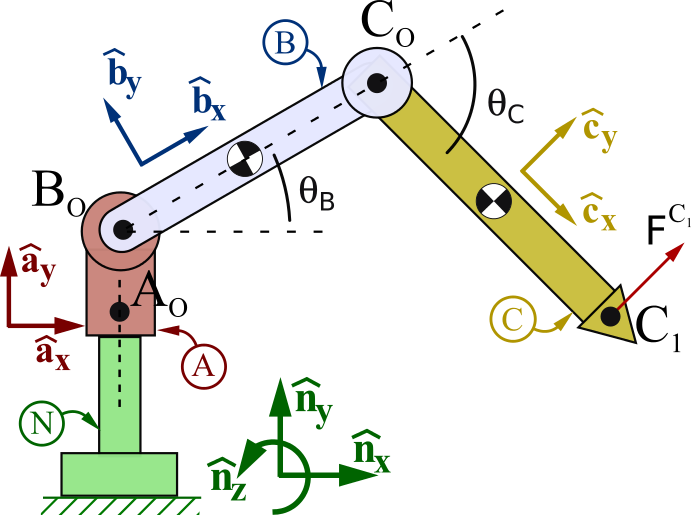
\includegraphics[width=0.99\linewidth]{robot_moment.png}
\end{minipage}
\\[0.45pc]
%-------------------------------
\smallerDescription[\small]{\begin{minipage}{0.32\linewidth}
{
   \rotationTableEmpty{a}{b}{\hspace{1.2cm}}
%   \simpleRotationZ{a}{b}{\thetaB}
}
\end{minipage}
\hfill
\begin{minipage}{0.28\linewidth}
{
%   \rotationTableEmpty{b}{c}{\hspace{1.3cm}}
    \simpleRotationNegativeZ{b}{c}{\thetaC}
}
\end{minipage}
\hfill
\begin{minipage}{0.32\linewidth}
{
   \rotationTable{a}{c}
   { ~\cos(\theta_B \minus[\!] \theta_C) }{  -\sin(\theta_B \minus[\!]  \theta_C) }{ 0 }
   { ~\sin(\theta_B \minus[\!] \theta_C) }{ ~~\cos(\theta_B \minus[\!]  \theta_C) }{ 0 }
   { 0                                   }{ 0                                     }{ 1 }
}
\end{minipage}}
\\[0.0pc]
%
\begin{enumerate}
\setlength{\itemsep}{0.25pc}
\item Complete the first rotation table \smallerDescriptionParens[\footnotesize]{above}.
      %
\item Express \posvec{A_o}{C_1} in terms of \uvecBasisxyz{a}.
      %The \uvecx{a} measure of \posvec{A_o}{C_1} is given to save you time.
      \\[0.0pc]\textbf{Result:}\\[-0.85pc]
      \begin{displaymath}
        \posvec{\origin{A}}{C_1} =
            \underline{\hidemath{[L_B \cos(\theta_B) + L_C \cos(\theta_B - \theta_C) ]}}~\uvecx{a}
            \plus[\;] \underline{\hidemath{}}~\uvecy{a}
            \plus[\;] \underline{\hidemath{}}~\uvecz{a}
      \end{displaymath}
      %
      \workspace{11.0pc}
      %
\clearpage
\item Calculate the moment of $\force{C_1}$ about \origin{C}.
      %
      \\[0.0pc]\textbf{Result:}\\[-0.85pc]
      %
      \begin{displaymath}
         \moment{\force{C_1}/\origin{C}} \equals[]\; \underline{\hidemath[1.45cm]{??}}\,\uvecx{c} \plus[\;]
         \underline{\hidemath[1.45cm]{??}}\,\uvecy{c} \plus[\;] \underline{\hidemath[1.45cm]{??}}\,\uvecz{c}
      \end{displaymath}
      %
      \workspace{15.0pc}
      %
%\clearpage
\item Calculate the moment of \force{C_1} about \origin{B}.
      %
      \\[0.0pc]\textbf{Result:}\\[-0.85pc]
      %
      \begin{displaymath}
         \moment{\force{C_1}/\origin{B}} \equals[]\; \underline{\hidemath[1.45cm]{??}}\,\uvecx{c} \plus[\;]
         \underline{\hidemath[1.45cm]{??}}\,\uvecy{c} \plus[\;] \underline{\hidemath[1.45cm]{??}}\,\uvecz{c}
      \end{displaymath}
      %
      \workspace{20.0pc}
      %
\end{enumerate}
%
\isolatedBuildFooter